% !TEX root = ../../homo_alg.tex

\newpage
\section{Resolutions}

\subsection{Projective Resolutions}

We now develop a homology theory that gives ``correction" terms for a functor, such as $- \otimes_R N, \Hom(-,N),\cdots$, not being left/right exact. For instance, the tensor functor is right exact but does not preserve all short exact sequences
\[
\cdots \ma{} A \otimes_R N \ma{} B \otimes_R N \ma{} C \otimes_R N \ma{} 0
\]
What terms exist on the left to make this sequence entirely exact? The key to filling in these terms is ``approximating" modules by projective or injective modules. Recall a presentation of an $R$-module $M$ is an expression of it as $M \cong F/K$, where $F$ is free and $K$ is a kernel. We do this by mapping a free module onto $M$:
\[
0 \ma{} K \ma{\subseteq} F \ma{\pi} M \ma{} 0
\]
We can then continue this process by finding a free module to map into $K$, which would then give a map from the new $F'$ to $F$
\[
\begin{tikzcd}
F' \arrow{dr} \arrow[dotted]{drr}{d_1} & & & & \\
0 \arrow{r} & K \arrow[swap]{r}{\subseteq} & F \arrow{r}{\pi} & M \arrow{r} & 0 
\end{tikzcd}
\] 
But then we have an exact sequence
\[
F_1 \ma{} F_0 \ma{} M \ma{} 0 
\]
Continuing this process again and again gives a ``full" exact sequence. We need only use projective modules to complete this process. 

\begin{dfn}[Projective Resolution]
A projective resolution of $R$-modules of $M$ is a complex $\dt{P}$ of projective modules together with a map to $M$, $P_0 \ma{\epsilon} M$, so that the augmented complex
\[
\cdots \ma{} P_1 \ma{} P_0 \ma{} M \ma{} 0 
\]
is exact. Equivalently, there is a quasi-isomorphism
\[
\begin{tikzcd}
\cdots \arrow{r} & P_2 \arrow{r} \arrow{d} & P_1 \arrow{r} \arrow{d} & P_0 \arrow{r} \arrow{d}{\epsilon} & 0 \arrow{d} \\
\cdots \arrow{r} & 0 \arrow{r} & 0 \arrow{r} & M \arrow{r} & 0 
\end{tikzcd}
\]
\end{dfn}

\begin{prop}[Existence]
In $R$-modules or any category in which all objects have projective mapping onto them, any module $M$ has a projective resolution. 
\end{prop}

Proof: Take a free module $F_0$ mapping onto $M$. Let $K_0= \ker \epsilon$. Take $F_1$ to be a free module mapping onto $K_0$ by $\pi_1$ and let $d_1=i\pi_1$. Proceed by induction taking $K_n= \ker d_n=\ker \pi_n$. Then the sequence is exact by construction. 
\[
\begin{tikzcd}
F_1 \arrow{r}{d_1} \arrow{dr}{\pi_1} & F_0 \arrow{r}{\epsilon} & M \arrow{r} & 0 \\
& K_0 \arrow{ru}{i} \arrow{dr} & & \\
0 \arrow{ur} & & 0 &
\end{tikzcd}
\]
\qed \\

\begin{ex}[Koszul complex]
Take $R=k[x,y]$ and let $M=R/(x,y) \cong k$, where $k$ is a field. 
\[
\begin{tikzcd}
0 \arrow{r} & R \arrow{r}{f=\begin{bmatrix} y \\ -x \end{bmatrix}} & R^2 \arrow{r}{[x\;\;y]} \arrow{d} & R \arrow{r}{\pi} & M \arrow{r} & 0 \\
 & K \arrow[swap]{ru}{f} & (x,y) \arrow{ur} & & & \\
 & 0 \arrow{ur} & & & & 
\end{tikzcd}
\]
Where $e_1 \mapsto x$ and $e_2 \mapsto y$. This is a famous resolution called the Koszul complex. 
\end{ex}

\begin{ex}
Take $R=k[x,y]/(xy)$ and $M$ to be the module $R/(x)$. 
\[
\begin{tikzcd}
\cdots \arrow{r} & R \arrow{r}{y} & R \arrow{r}{x} & R \arrow{r} \arrow{d} & R \arrow{r} \arrow{d} & R \arrow{r}{\pi} & M \arrow{r} &0 \\
& & & (y) \arrow{ur} & (x) \arrow{ur} & &
\end{tikzcd}
\]
\end{ex}

\begin{thm}[Comparison Theorem]
Given a map $f': M \to N$ and complexes 
\[
\begin{tikzcd}
\cdots \arrow{r} & P_2 \arrow{r} & P_1 \arrow{r} & P_0 \arrow{r}{\epsilon} & M \arrow{d}{f'} & \\
\cdots \arrow{r} & Q_2 \arrow{r} & Q_1 \arrow{r} & Q_0 \arrow{r}{\eta} & N \arrow{r} & 0 
\end{tikzcd}
\]
with each $P_i$ projective and the bottom row exact, then the map $f'$ can be lifted, i.e. $\eta f=f' \epsilon$ to a chain map $\dt{P} \ma{f} \dt{Q}$ and any two lifts are homotopic. 
\end{thm}

Proof: We do this by induction. Assume we have a diagram
\[
\begin{tikzcd}
0 \arrow{r} & Z_0 \arrow{r} \arrow[dotted]{d}{f_0} & P_0 \arrow[dotted]{d}{f_0} \arrow{r}{\epsilon} & M \arrow{d}{f'} \\
0 \arrow{r} & Z_0' \arrow{r} & Q_0 \arrow{r}{\eta} & N
\end{tikzcd}
\]
As $P_0$ is projective and $\eta$ is surjective, there is a $f_0$ such that the diagram
\[
\begin{tikzcd}
\phantom{x} & P_0 \arrow[dotted]{dl}{f_0} \arrow{d}{f' \epsilon} \\
Q_0 \arrow{r}{\eta} & N 
\end{tikzcd}
\]
We have $\eta f_0 =f'\epsilon$ so that the last square commutes. Therefore, we have a map $Z_0 \to Z_0'$ using a previous lemma. Then $f_0(Z_0) \subseteq Z_0'$ so $f_0$ restricts to a map $Z_0 \to Z_0'$.

Now if you have constructed the maps for all $I \leq n$, then we have a commutative diagram
\[
\begin{tikzcd}
P_{n+1} \arrow{rr}{d} \arrow{dr}{d} \arrow[dotted]{dd} & & P_n \arrow{rr}{d} \arrow{dd}{f_n} & & P_{n-1} \arrow{dd}{f_{n-1}} \\
 & Z_n \arrow[hook]{ur} & & & \\
Q_{n+1} \arrow{rr}{d} \arrow{drr}{d'} & & Q_n \arrow{rr}{d} & & Q_{n-1} \\ 
 &  & Z_n' \arrow[hook]{u}& & \\
\end{tikzcd}
\]
As the right square commutes, $f_n$ restricts to give a map $Z_n=\ker d \to Z_n'= \ker d'$. Note that $\im d: P_{n+1} \to P_n \subseteq Z_n$ as $d^2=0$. Likewise in the bottom row, $\im d' \subseteq Z_n'$ as $\dt{Q}$ is exact: $\im d'=Z_n'$ so that the map is surjective onto $Z_n'$. This yields a diagram
\[
\begin{tikzcd}
\phantom{x} & P_{n+1} \arrow[dotted]{dl}{f_{n+1}} \arrow{d}{f_n d} \\
Q_{n+1} \arrow{r}{d'} & Z_n'
\end{tikzcd}
\]
Since $P_{n+1}$ is projective, we get a map $f_{n+1}: P_{n+1} \to Q_{n+1}$ such that the triangle commutes -- forcing commutativity of the square. Therefore, we obtain the result via induction. 

We need only see that this map is unique up to homotopy. We do this by induction as well. Suppose $g: \dt{P} \to \dt{Q}$ is another lift of $f'$. We want to show that given another lift $g$, we have $f \simeq g$, i.e. $f-g \simeq 0$. Let $h=f-g$. Note that $h$ is a difference so it is a lift $M \to N$, $f'-f'=0$ so it is a lift of 0. 
\[
\begin{tikzcd}
\phantom{x} & & &  & 0 \\
 & & & M \arrow{ur} & \\
\cdots \arrow{r} & P_1 \arrow{r} \arrow{d}{h_1} & P_0 \arrow{ur}{\epsilon} \arrow{d}{h_0} \arrow{dl} \arrow{r} & 0 \arrow{r} \arrow{d}{0} \arrow{dl}{s_{-1}} & 0 \arrow{d} \arrow{dl}{s_{-2}} \\
\cdots \arrow{r} & Q_1 \arrow{r}{d'} & Q_0 \arrow{r} \arrow{dr} & 0 \arrow{r} & 0 \\
 & & & N \arrow{dr} &  \\
 & & &  & 0 
\end{tikzcd}
\]
For $n<0$, we know that $s_n=0$. We need find a map $s_0: P_{0\cdot} \to Q_{0\cdot}$. We need $h_0: \underbrace{sd}{0}+ds$. Let $Z_0'=\ker \eta$. As $\dt{Q} \to N \to 0$ is exact, we know that $\im d'=\ker \eta=Z_0'$. 
 \[
 \begin{tikzcd}
 \phantom{x} & &  & 0\\
  & & M \arrow{ur} & \\
 P_1 \arrow{r}{d} \arrow{d}{h_1} & P_0 \arrow{ur}{\epsilon} \arrow{r} \arrow[dotted]{dl}{s_0} \arrow{d}{h_0} & 0 & \\
 Q_1 \arrow{r}{d'} \arrow{dr}{d'} & Q_0 \arrow{dr}{\eta} \arrow{r} & 0 & \\
   & Z_0 \arrow[hook]{u} & N \arrow{dr} & \\
    &  &  & 0\\
 \end{tikzcd}
 \]
Now $\eta h_0=0$. So $\im h_0 \subseteq \ker \eta=Z_0'$. Then we have a diagram
\[
\begin{tikzcd}
\phantom{x} & P_0 \arrow[dotted]{dl} \arrow{dr}{h_0} & \\
Q_1 \arrow{rr}{d'} & & Z_0'
\end{tikzcd}
\]
As $P_1$ is projective, there is a map $s_0: P_0 \to Q_1$ such that the triangle commutes. This completes the base step. We now proceed with the induction argument. Given $s_i$ with $i \leq n$ and $h_n=d's_n+s_{n-1}d$.
\[
\begin{tikzcd}
P_{n+2} \arrow{d}{h_{n+2}} \arrow{r} & P_{n+1} \arrow{r} \arrow{d}{h_{n+1}} \arrow[dotted]{dl}{s_{n+1}} & P_n \arrow{r} \arrow{d}{h_n} \arrow{r}{d} & P_{n-1} \arrow{d}{h_{n-1}} \arrow{dl}{s_{n-1}} \\
Q_{n+2} \arrow{r} & Q_{n+1} \arrow{r} & Q_n \arrow{r}{d'} & Q_{n-1} 
\end{tikzcd}
\]
We want to find an $s_{n+1}$ such that $h_{n+1}=d's_{n+1} + s_nd$. That is, $h_{n+1}-s_nd=d's_{n+1}$. Then $Z_{n+1}' =\ker d' \subseteq Q_{n+1}$. By exactness, $\im d' =Z_{n+1}'$ so that $d'$ restricts to a surjection $Q_{n+2} \ma{d'} Z_{n+1}'$. 
\[
\begin{split}
d'(h_{n+1}-s_nd) &=d'h_{n+1}-d's_nd \\
&=d'h_{n+1}-(h_n-s_{n-1}d)d \\
&=d'h_{n+1}-h_nd+s_{n-1}d^2 \\
&=0
\end{split}
\]
so that $\im(h_{n+1}-s_nd) \subseteq Z_{n+1}'$. Then we have a diagram
\[
\begin{tikzcd}
\phantom{x} & P_{n+1} \arrow[dotted]{dl}{s_{n+1}} \arrow{d}{h_{n+1}-s_nd} \\
Q_{n+2} \arrow{r}{d'} & Z_{n+1}'
\end{tikzcd}
\]
\qed \\

\begin{cor}
A projective resolution of a module is unique up to homotopy, i.e. any two projective resolutions are homotopy equivalent. 
\end{cor}

Proof: Let
\[
\begin{tikzcd}
P_0 \arrow{r} & M \arrow{d}{1_M} \\
Q_0 \arrow{r} & M 
\end{tikzcd}
\]
be two projective resolutions of $M$. By the Comparison Theorem, there is a lift $P_{0\cdot} \ma{f} \dt{Q}$, $\dt{Q} \ma{g} \dt{P}$ of the identity map. Note that both $fg: \dt{Q} \to \dt{Q}$ and $1_{\dt{Q}}$ are both lifts of $1_M$. So by uniqueness, $fg \simeq 1_{\dt{Q}}$ and similarly $gf \simeq 1_{\dt{P}}$. 

The following lemma is useful for building resolutions for extensions.

\begin{lem}[Horseshoe Lemma]
Given a short exact sequence of $R$-modules
\[
0 \ma{} M' \ma{} M \ma{} M'' \ma{} 0
\]
and projective resolutions $\dt{P}' \to M'$, $\dt{P}'' \to M''$, then one can build a projective resolution $\dt{P} \to M$ with $P_n= P_n' \oplus P_n''$ and differential $d$ of the form
\[
\begin{matrix}
P_n' & \begin{bmatrix} d' & * \\ 0 & d'' \end{bmatrix} & P_{n-1}' \\
\oplus & \ma{} & \oplus \\
P_n'' & & P_{n-1}''
\end{matrix}
\]
so as to get an exact sequence
\[
0 \ma{} \dt{P}' \ma{i_1} \dt{P} \ma{\pi_2} \dt{P}'' \ma{} 0
\] 
\end{lem}

Proof: 
\[
\begin{tikzcd}
\phantom{x}  & \arrow{d} & \arrow{d} & \arrow{d}  & \\
0 \arrow{r} & P' \arrow{d} \arrow{r} & P_1' \oplus P_1'' \arrow{d} \arrow{r} & P_1'' \arrow{d} & \\
0 \arrow{r} & P_0' \arrow{d}{\epsilon'} \arrow{r}{i_1} & P_0' \oplus P_0'' \arrow[dotted]{d} \arrow{r}{\pi_2} & P_0'' \arrow{r} \arrow{d}{\epsilon''} \arrow[dotted]{dl}{\theta} & 0 \\
0 \arrow{r} & M' \arrow{d} \arrow{r}{i} & M \arrow{r}{\pi} & M'' \arrow{d} \arrow{r}& 0 \\
& 0 & & 0 & 
\end{tikzcd}
\]
Since $P_0''$ is projective and $\pi$ is onto, there is a map $\theta: P_0'' \to M$ such that $\pi \theta= \epsilon''$. This map $\theta$ with $i \epsilon': P_0' \to M$ gives a map $\epsilon: P_0' \oplus P_0'' \to M$ given by $(a,b) \mapsto i \epsilon(a)+\theta(b)$. By the Snake Lemma, $\coker \epsilon=0$ so that $\epsilon$ is onto. 
Then the sequence
\[
0 \ma{} \ker \epsilon' \ma{} \ker \epsilon \ma{} \ker \epsilon'' \ma{\delta} 0 
\]
is exact. Repeat the argument to 
\[
\begin{tikzcd}
0 \arrow{r} & P_1' \arrow{r}{i_1} \arrow{d}{d'} & P_1' \oplus P_1'' \arrow[dotted]{d} \arrow{r}{\pi_2} & P_1'' \arrow{r} \arrow{d}{d''} & 0 \\
0 \arrow{r} & \ker \epsilon' \arrow{d} \arrow{r} & \ker \epsilon & \ker \epsilon'' \arrow{r} \arrow{d} & 0 \\
& 0 & 0 & 0 & 
\end{tikzcd}
\]
Since $P' \ma{\epsilon'} M'$ and $P'' \ma{\epsilon''} M''$ are resolutions, we can repeat the argument above to find that the squares commute and
\[
d= \begin{bmatrix} d' & * \\ 0 & d'' \end{bmatrix} 
\]

\subsection{Injective Resolutions} 

Really that any $R$-module $M$ can be indebted into an injective $R$-module. 
\[
M \hookrightarrow E(M)
\]
where $E(M)$ is the smallest injective $R$-module containing $M$, i.e. the injective hull/envelope. 

\begin{dfn}[Injective Resolution]
Given an $R$-module $M$, an injective resolution of $M$ is an exact sequence
\[
0 \ma{} M \ma{} I^0 \ma{} I^1 \ma{} I^2 \ma{} \cdots
\]
where each $I^i$ is an injective $R$-module. 
\end{dfn}

We need justify the existence of an injective resolution for any $R$-module $M$. We can embed $M$ into an injective $R$-module, take the cokernel of the map and embed it into an injective $R$-module $I'$. Then we can take the cokernel of this map and continue this process:
\[
\begin{tikzcd}
0 \arrow{r} & M \arrow{r}{\epsilon} & I^0 \arrow{rr}{d^0=i \pi} \arrow{dr}{\pi} & & I' \\
& & & \coker \epsilon \arrow{ur}{i} & 
\end{tikzcd}
\]

\begin{thm}[Comparison Theorem]
Given a map $M \ma{f'} N$ and complexes
\[
\begin{tikzcd}
0 \arrow{r} & M \arrow{d}{f'} \arrow{r} & J^0 \arrow{r} \arrow[dotted]{d} & J^1 \arrow{r} \arrow[dotted]{d} & J^2 \arrow{r} \arrow[dotted]{d} & \cdots \\
0 \arrow{r} & N \arrow{r} & I^0 \arrow{r} & I^1 \arrow{r} &  I^2 \arrow{r} & \cdots 
\end{tikzcd}
\]
with each $I^n$ an injective $R$-module and $0 \to M \to \dt{J}$ exact, $f'$ can be lifted to a cochain map $f: J^\cdot \to I^\cdot$ uniquely up to homotopy. 
\end{thm}

Proof: This follows mutatis mutandis from the proof of the Comparison Theorem for Projective Resolutions. \qed \\

\begin{rem}
\emph{\textbf{From now on, functors will be assumed to be additive!}}
\end{rem}

We now generalize the concept of injective and projective resolutions to a type of functor: derived functors. These were first developed by, among others, Grothendieck and made widely accessible in the book by Cartan and Eilenberg. 

\subsection{Left Derived Functors}

\begin{dfn}[Left Derived Functor]
Let $F: \cA \to \cB$ be a \emph{right} exact functor between abelian categories. Given a short exact sequence,
\[
0 \ma{} A \ma{} B \ma{} C \ma{} 0
\]
we obtain an exact sequence
\[
? \ma{} F(A) \ma{} F(B) \ma{} F(C) \ma{} 0
\]
If $\cA$ has projective resolutions, define the left derived functor $L_nF$ of $F$ for $n \geq 0$ by the following: if $M \in \cA$, choose a projective resolution $\dt{P} \to M$ and defined $L_nF(M)= H_n(F(\dt{P}))=H_n(\cdots \ma{F(d)} F(P_1) \ma{F(d)} F(P_0) \ma{} 0)$. 
\end{dfn}

There is one one particular type of left functor of great enough importance to warrant its own name and separate definition:

\begin{dfn}[Tor]
The function $F(-)= - \otimes_R N$ is a right exact functor from \textbf{R-mod} to $\Z$-mod. Its left derived functors are called $\Tor^R_n(-,N) \defeq L_nF(-)$, i.e. for any $M$
\[
\Tor_n^R(M,N)= L_nF(M)=H_n(F(\dt{P}))
\]
where $\dt{P} \to M$ is a projective resolution; that is, the homology groups of 
\[
\cdots \ma{d \otimes 1} P_1 \otimes N \ma{d \otimes 1} P_0 \otimes N \ma{} 0 
\]
\end{dfn}

\begin{ex}
Let $R$ be a ring and $f$ a nonzero divisor in $R$. Let $M=R/(f^2)$ and $N=R/(f)$. We compute $\Tor_n^R(M,N)$. Take the projective resolution of $M$
\[
\begin{tikzcd}
\cdots \arrow{r} & 0 \arrow{r} & 0 \arrow{r} & R' \arrow{rr}{f^2} \arrow{dr} & & R' \arrow{r}{\pi} & M \arrow{r} & 0 \\
& & & & (f^2) \arrow[hook]{ur} & & & 
\end{tikzcd}
\]
Note that if $xf^2=0$, then $x=0$ as $f$ is a nonzerodivisor. Now apply the functor $- \otimes_R N$:
\[
\begin{tikzcd} 
0 \arrow{r} & R \otimes_R N \arrow{r}{f^2 \otimes 1} \arrow{d}{\sim} & R \otimes_R N \arrow{r} \arrow{d}{\sim} & 0 \\
& N \arrow{r}{f^2=0} & N & 
\end{tikzcd}
\]
So we have
\[
\begin{split}
\Tor_0^R(M,N)&=H_0(\text{complex})=R/(f)/0=R/(f) \\
\Tor_1^R(M,N)&=H_1(\text{complex})=R/(f)/0=R/(f) \\
\Tor_n^R(M,N)&=0 \;\;\;\;\; n \geq 2
\end{split}
\]
\end{ex}

However, there is a problem with the above example: we did not justify why the Tor groups would not be different had we chosen any other projective resolution. 

\begin{prop}
\begin{enumerate}[(i)]
\item $L_nF$ is well defined; that is, $L_nF$ is independent of the choice of projective resolution. 
\item $L_nF$ is a functor and given $f: M \to K$, we get $L_n(F): L_nF(M) \to L_nF(K)$
\item $L_0F=F$
\item For any short exact sequence $0 \to M' \to M \to M'' \to 0$, there exist connecting maps $\delta_n$ and a long exact sequence
\[
\begin{tikzcd}
  \cdots \rar   & L_{n+1}F(M') \rar & L_{n+1}F(M) \rar & L_{n+1}F(M'')
          \ar[out=0, in=180, looseness=2, overlay]{dll}{\delta_{n+1}}   & \\
        & L_nF(M') \rar & L_nF(M) \rar & L_nF(M'')
          \ar[out=0, in=180, looseness=2, overlay]{dll}{\delta_n}   & \\
        & L_{n-1}F(M') \rar & L_{n-1}F(M) \rar & \cdots
          \ar[out=0, in=180, looseness=2, overlay]{dll}{\delta_1}   & \\
        & L_0F(M')  \rar & L_0F(M)\rar & L_0F(M'') \rar & 0
\end{tikzcd}
\]
\end{enumerate}
such that the $\delta_n$ are natural; that is, if for any map of short exact sequences
\[
\begin{tikzcd}
0 \arrow{r} & M' \arrow{r} \arrow{d} & M \arrow{d} \arrow{r} & M'' \arrow{r} & 0 \\
0 \arrow{r} & K' \arrow{r}  & K  \arrow{r} & K'' \arrow{r} & 0 
\end{tikzcd}
\]
the ``obvious" ladder diagram of the two long exact sequences and maps between them commutes, i.e. for all $n$ the following diagram commutes:
\[
\begin{tikzcd}
L_nF(M'') \arrow{d} \arrow{r}{\delta_0} & L_{n-1}F(M') \arrow{d} \\
L_nF(K'') \arrow{r}{\delta_n} & L_{n-1}F(K')
\end{tikzcd}
\]
% Any collection of functots $\{\sigma_n\}_{n \geq 0}$ satisfying (ii) and (iv)
\end{prop}

\noindent Proof: 
\begin{enumerate}[(i)]
\item If $\dt{P} \to M$ and $\dt{P}' \to M$ are two projective resolutions of $M$, then by the Comparison Theorem, they are homotopy equivalent. So there exist lifts of $1_M$
\[
\begin{tikzcd}
\dt{P} \arrow[yshift=1ex]{r}{f} & \dt{P}' \arrow[yshift=-1ex]{l}{g}
\end{tikzcd}
\]
such that $fg \simeq 1_{\dt{P}'}$ and $gf \simeq 1_{\dt{P}}$. Applying the function $F(-)$, we obtain $F(fg) \simeq F(1)$ via the homotopy $F(s)$, where $s$ is the homotopy for $fg \simeq 1$. Then we have $F(f) F(g) \simeq 1_{\dt{P}'}$ and likewise $F(g)F(f) \simeq 1_{\dt{P}}$. So $F$ applied to the complexes gives a homotopy equivalence. Then this must induce the same map on homotopy so that $H_nF(f) H_nF(g) = H_n(1)=1$. Therefore, we have $H_nF(g)H_nF(f)=1$ so that $H_nF(f)$ is an isomorphism. But then $H_nF(f): H_nF(\dt{P})=L_nF(M) \to H_nF(\dt{P}')=L_nF(M)$ is an isomorphism. 

\item This part follows similarly to (i). Let $M \ma{f} K$. Let $\dt{P} \to M$ and $\dt{Q} \to K$ be projective resolutions of $M$ and $K$, respectively. By the Comparison Theorem, we then get a lift of $\dt{P} \ma{'f'} \dt{Q}$. Applying the function $F$, we get a chain map $F(\dt{P}) \ma{F(f)} F(\dt{Q})$. Hence, we get an induced map on homology: $L_nF(M) \to L_nF(K)$.

\item Simply compute $L_0F(M)$ given that $\dt{P} \to M$ is a projective resolution.
\[
L_0F(M)=H_0(F(\dt{P}))=\coker(F(P_1) \to F(P_0))=F(M)
\]
since $F(P_1) \to F(P_0) \to M \to 0$ is exact. 

\item Let
\[
0 \ma{} M' \ma{} M \ma{} M'' \ma{} 0
\]
be a short exact sequence. By the Horseshoe Lemma, there is a projective resolution fitting in a diagram
\[
\begin{tikzcd}
0 \arrow{r} & \dt{P}' \arrow{d}{\epsilon'} \arrow{r} & \dt{P} \arrow{d}{\epsilon} \arrow{r} & \dt{P}'' \arrow{r} \arrow{d}{\epsilon''} & 0 \\
0 \arrow{r} & M' \arrow{r} & M \arrow{r} & M'' \arrow{r} & 0
\end{tikzcd}
\]
with exact rows (in fact, this diagram is even split). Applying $F$ preserves exactness in each row (check this, use the ``splitness"). Then we have
\[
\begin{tikzcd}
0 \arrow{r} & F\dt{P}' \arrow{d} \arrow{r} & F\dt{P} \arrow{d} \arrow{r} & F\dt{P}'' \arrow{d} \arrow{r} & 0 \\
0 \arrow{r} & FM' \arrow{r} & FM \arrow{r} & FM'' \arrow{r} & 0
\end{tikzcd}
\]
Now we use the long exact sequence on homology and we are done. [Naturality has yet to be proven but for this see Weibel.]
\end{enumerate}
\qed \\

\begin{prop}
$F$ is a right exact additive functor if and only if $L_nF=0$ for all $n>0$ if and only if $L_1F=0$.
\end{prop}

\noindent Proof: The reverse direction follows from the definition and the forward direction follows easily from the long exact sequence. \qed \\

\begin{dfn}[$\delta$-functor]
A $\delta$-functor is a collection $\{T_n\}_{n \geq 0}$ of additive functors such that (iv) holds. That is for all exact
\[
0 \ma{} A \ma{} B \ma{} C \ma{} 0
\]
there is a natural $\delta_n$'s such that 
\[
 \cdots \ma{} T_1A \ma{} T_1B \ma{} T_1C \ma{\delta} T_0A \ma{} T_0B \ma{} T_0C \ma{} 0
\]
is a long exact sequence. The functor $\delta$ is called universal if given any other $\delta$-functor, $\{\delta_n\}$ and natural transformation $S_0 \to T_0$, there is a unique map of $\delta$-functors from
\[
\{S_n\} \ma{\{f_n\}} \{T_n\}
\]
that commute with the $\delta$'s. 
\end{dfn}

\begin{cor}
Any two universal $\delta$-functors, $\{T_n\}, \{T_n'\}$ with isomorphic $T_0,T_0;$ are isomorphic, i.e. $T_n \cong T_n'$ and the isomorphisms commute with the $\delta$'s.
\end{cor}

\begin{thm}
Given a right exact $F$, $\{L_nF\}_{n \geq 0}$ are a universal $\delta$-functor (so they are unique).
\end{thm}

Recall $\tor_n^R(M,N)=L_nF$ of functor $F(-)= - \otimes_R N$.

\subsection{Balancing Tor}

There are two derived functors we can associate to 
\[
M,N \ma{} M \otimes_R N
\]
Namely, $F(-)= - \otimes_r N$ and $G(-)= M \otimes_R -$. We have $F(M)=G(N)$. What about $L_nF(M)$ and $L_nG(N)$? These behave as expected; however, the proof needs many details. We attend to the proof first then fill in the necessary lemmas afterwards.

\begin{thm}
If $\dt{P} \ma{\ep} M$ and $\dt{Q} \ma{\eta} N$ are projective resolutions, then
\[
H_N(\dt{P} \otimes N) \cong H_n(\tot(\dt{P} \otimes Q_0)) \cong H_n(M \otimes \dt{Q}) = \tor_n^R(M,N)
\]
(note that the $\tot$ is often dropped).
\end{thm}

\noindent Proof: Let $\dt{P} \to M$ be a projective resolution. That is
\[
\cdots \ma{} P_2 \ma{} P_1 \ma{} P_0 \ma{\ep} M 
\]
is exact or equivalently
\[
\begin{tikzcd}
\cdots \arrow{r} & P_2 \arrow{r} \arrow{d} & P_1 \arrow{d} \arrow{r} & P_0 \arrow{r} \arrow{d}{\ep} & 0 \\
\cdots \arrow{r} & 0 \arrow{r} & 0 \arrow{r} & M \arrow{r}{=} & M
\end{tikzcd}
\]
is a quasi-isomorphism. Hence, we have a map of bicomplexes: 

\begin{figure}[h] 
   \centering
   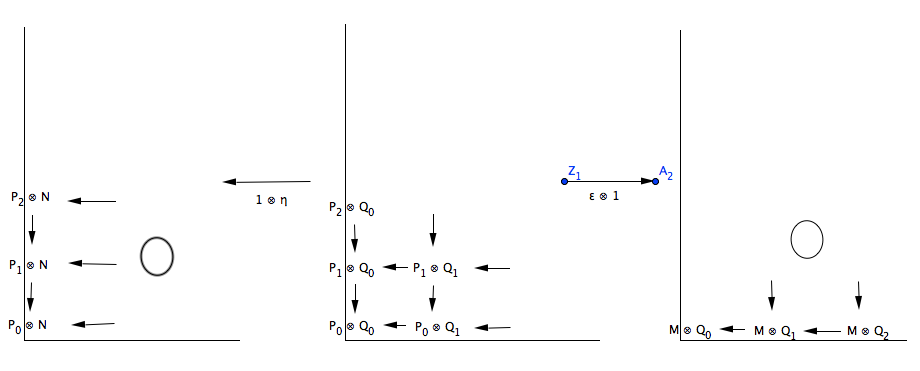
\includegraphics[width=4in]{images/bicom.png} 
\end{figure}

We want to show that $\tot(1 \otimes \eta)$ is a quasi-isomorphism, likewise for $\tot(\ep \otimes 1)$. However, the latter follows mutatis mutandis. By Lemma \ref{lemone}, it is enough to show that $1 \otimes \eta$ is a quasi-isomorphism on each row. By Lemma \ref{lemthree}, it will follow since each $P_n$ is projective, hence flat. So $P_n \otimes -$ is an exact functor so it preserves quasi-isomorphisms (show this). \qed \\

\begin{lem} \label{lemone} 
If $A_{\cdot \cdot} \ma{f} B_{\cdot \cdot}$ is a map of first quadrant bicomplexes (with arrows towards the origin or away from the origin) such that the map on each row/column is a quasi-isomorphism, then $\tot(A_{\cdot \cdot} \ma{\tot(f)} \tot(B_{\cdot \cdot})$ is a quasi-isomorphism. 
\end{lem}

\noindent Proof (Sketch): By taking cones of $f$ on the rows, one obtains a bicomplex, say $C_{\text{row/col}}(f)$. Note, $f$ is a quasi-isomorphism on the rows so that $C_{\text{row/col}}(f)$ is exact in each row/column. Also,
\[
0 \ma{} B_{\cdot \cdot} \stackrel{i}{\hra} C_{\text{row/col}}(f) \ma{\pi} A_{\cdot \cdot}[-1] \ma{} 0
\]
is exact. Then
\[
0 \ma{} \tot(B) \ma{} \tot(C_{\text{row/col}}) \ma{} \tot(A_{\cdot \cdot})[-1] \ma{} 0
\]
is exact. But the middle term is precisely $C(\tot(f))$. By Lemma \ref{lemtwo}, the sequence is exact so $\tot(f)$ is a quasi-isomorphism. \qed \\

\begin{lem} \label{lemtwo}
If $\dt{C}$ is a first quadrant bicomplex with exact rows (or columns) then $\tot(C_{\cdot \cdot})$ is exact. 
\end{lem}

\noindent Proof:
\begin{figure}[h] 
   \centering
   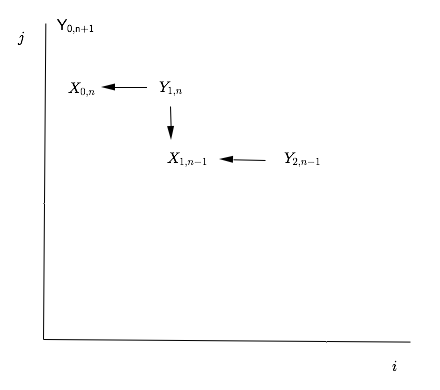
\includegraphics[width=3in]{images/arrows.png} 
\end{figure}
Let $X=(X_{ij}) \in \oplus_{i+j=n} C_{ij}$ be a cycle in $\tot(C)$, i.e. for each $i$, $(-1)^id(X_{i,n-i})+d'(X_{i-1,n-(i-1)})=0$, where $(-1)^id$ are the downwards maps in the complex and $d'$ are the left arrows in the complex. Start at the upper left. Let $Y_{0,n+1}=0$. Since $d'(X_{0,n})=0$ and the rows are exact, there is a $Y_{1,n}$ such that $d'(Y_{1,n})=X_{0,n}$. Check that $X_{1,n-1}-(-d(Y_{1,n})) \in \ker d'$. Since the rows are exact, there is a $Y_{2,n-1} \in d'(Y_{2,n-1})=X_{1,n-1}+d(Y_{1,n})$. Then ``$d$" of the $Y$'s so far are $X_{1,n-1}$. Continue this process by induction. This induction must end as the complex is 1st quadrant (at the most when it hits the axis). So ``$d$" of the $Y$'s is $(X_{ij})_{i+j=n}$, so $(X_{ij})$ is a boundary. \qed \\

\begin{lem} \label{lemthree}
Let $\dt{A} \ma{f} \dt{B}$ be a chain map (map of complexes). If $f$ is a quasi-isomorphism and $P$ is flat, then $P \otimes \dt{A} \ma{1 \otimes f} P \otimes \dt{B}$ is a quasi-isomorphism. 
\end{lem}

\noindent Proof: Suppose that $A \ma{f} B$ is a quasi-isomorphism. Then $C(f)$ is exact so that as $P$ is flat, $P \otimes \dt{C(f)}$ is exact. But this is isomorphic to $C(1 \otimes f)$. Then $1 \otimes f$ is a quasi-isomorphism. \qed \\

The same proof works for $F(-)$ instead of $P \otimes -$ if $F$ is an exact functor. Suppose
\[
0 \ma{} A \ma{} B \ma{} C \ma{} 0
\]
is an exact sequence. Then we get the exact sequence
\[
A \otimes N \ma{} B \otimes N \ma{} C \otimes N \ma{} 0
\]
We get a similar sequence for $M \otimes -$. 

\begin{cor}
We have two long exact sequences for
\[
\tor(M,N)=H_n(\dt{P} \otimes N) = H_n(M \otimes \dt{Q})
\]
\end{cor}

\subsection{Right Derived Functors}

\begin{dfn}
Let $F: \cA \to \cB$ be a left exact functor, where $\cA$ and $\cB$ are abelian and $F$ is additive. If $\cA$ has injective resolutions, then we can define a right derived functor by taking $N \in \cA$ and take injective resolution $N \to I^{\cdot}$:
\[
R^nF(N) \defeq H^n(F(I^{\cdot}))
\]
\end{dfn}

This is the same construction as before applied to $F^{\text{op}}: \cA^{\text{op}} \to B^{\text{op}}$. That is, $F$ is left exact if and only if $F^{\text{op}}$ is right exact. Similarly, we have injective resolutions in $\cA$ if and only if we have projective resolutions in $A^\text{op}$. So we have an automatic proof of:

\begin{thm}
\begin{enumerate}[(i)]
\item $R^nF: \cA \to \cB$ is well-defined (independent of the choice of injective resolution) and is a functor for all $n$
\item $R^0F=F$
\item if $0 \to A \to B \to C \to 0$ is exact, then there are a functorial, i.e. natural, maps $\delta^n$ such that we get a long exact sequence
\[
0 \ma{} R^0F(A) \ma{} R^0F(B) \ma{} R^0F(C) \ma{\delta} R^1F(A) \ma{} R^1F(B) \ma{} R^1F(C) \ma{\delta} \cdots
\]
\end{enumerate}
\end{thm}

The major example will be the Ext functor. Let $M,N \in R-\text{mod}$. Let $F(-)\defeq \Hom_R(M,-)$. Then $F$ is covariant and left exact. These right derived functors are called the Ext functors.
\[
\Ext_R^n(M,N)=R^nF(N)
\]
i.e. $H^n(\Hom(M,\dt{I}))$. 

\begin{ex}
$\Ext_{\Z}^n(\Z/k\Z,\Z)$ for $k \geq 2$. Recall over a PID, injective is equivalent to divisible. So we have an injective resolution of $\Z$
\[
0 \ma{} \Z \hra \Q \ma{} \Q/\Z \ma{} 0
\]
where $I^0=\Q$ and $I^1=\Q/\Z$, which are divisible so they are injective $\Z$-modules. Then we have
\[
0 \ma{} \Hom_{\Z}(\Z/k\Z,\Q)=0 \ma{} \Hom_{\Z}(\Z/k\Z,\Q/\Z) \ma{} 0
\]
So then we have
\[
\begin{split}
\Ext^0_{\Z}(\Z/k\Z,\Z) &= H^0(\text{above})=0/0=0 \\
\Ext^1_{\Z}(\Z/k\Z,\Z) &= H^1(\text{above})=\Hom_{\Z}(\Z/k\Z,\Q/\Z)/0
\end{split}
\]
where the maps in $\Ext_{\Z}^1$ are given by $\overline{1} \mapsto p/q$ with $(p,q)=1$ such that $k \overline{p/q}=0 \in \Z$ so that $q \mid k$ which is $\{p/q \in \Q/\Z \;|\; kp/q \in \Z\}$. 
\end{ex}

Note that $\Ext_R^0(M,N)=\Hom_R(M,N)$.

\subsection{Contravariant Functors}

If $F: \cA \to \cB$ is contravariant and left exact. We get $F^1: \cA^{\text{op}} \to \cB$ is contravariant. So this is still left exact so we can use the construction from before. So $F'$ has right derived functors which are 
\[
R^nF'(M) \defeq H^n(F'(\text{injective resolution of }M \text{ in }\cA))
\]
which is $H^n(F(\text{projective resolution of }M\text{ in }\cA))=R^nF(M)$. 

\begin{ex}
$F(-)=\Hom_R(-,N)$ is left exact. This gives $R^nF(M)=H^n(\Hom(\dt{P},N))$, where $\dt{P}$ is a projective resolution of $M$. 
\end{ex}

\subsection{Balancing Ext}

We have two derived functors to associate to $M,N \to \Hom_R(M,N)$. Namely, $\Hom(M,-)$ and $\Hom_R(-,N)$. 

\begin{thm}
If $N \ma{\eta} I^{\cdot}$ is an injective resolution and $\dt{O} \ma{\ep} M$ is a projective resolution
\[
\Ext_R^0(M,N)=H_n(\Hom(M,I^{\cdot})) \cong H_n(\tot(\Hom(\dt{P},I^{\cdot}))) \cong H_n(\Hom(\dt{P},N))
\]
\end{thm}

\begin{ex}
We redo the example from before. Take $\Ext_{\Z}^n(\Z/k\Z,\Z)$. So instead of taking a projective resolution of $\Z/k\Z$, we take a projective resolution of $\Z/k\Z$
\[
0 \ma{} \Z \ma{k} \Z \ma{} \Z/k\Z \ma{} 0
\]
where $P_1=\Z$ and $P_0=\Z$. Then we have $\Ext^n=H^n(\Hom_{\Z}(\dt{P},\Z))$ so we have
\[
0 \ma{} \Hom_{\Z}(\Z,\Z) \ma{k^*} \Hom_{\Z}(\Z,\Z) \ma{} 0 
\]
which is
\[
0 \ma{} \Z \ma{k} \Z \ma{} 0
\]
So that $\Ext_{\Z}^0(\Z/k\Z,\Z)=0$ and $\Ext_{\Z}^1(\Z/k\Z,\Z)=\Z/k\Z$, which is the subgroup $\langle 1/k \rangle$ of $\Q/\Z$. 
\end{ex}

\begin{cor}
If 
\[
0 \ma{} A \ma{} B \ma{} C \ma{} 0
\]
is exact. There are two types of long exact sequences
\[
0 \to \Hom(M,A) \to \Hom(M,B) \to \Hom(M,C) \ma{\delta} \Ext^1(M,A) \to \Ext^1(M,B) \to \Ext^1(M,C) \ma{\delta} \cdots
\]
and the long exact sequence
\[
0 \to \Hom(C,M) \to \Hom(B,M) \to \Hom(A,M) \ma{\delta} \Ext^1(C,M) \to \Ext^1(C,M) \to \Ext^1(A,M) \ma{\delta} \cdots
\]
\end{cor}

Note that since $\Tor$ and $\Ext$ are balanced, there is another way to get the same long exact sequence (avoiding the Horseshoe Lemma). For example for $\Ext$, if we have the exact sequence
\[
0 \ma{} A \ma{} B \ma{} C \ma{} 0
\]
and an $R$-module $M$, we take a projective resolution $\dt{P} \to M$ of $M$, then
\[
0 \to \Hom(\dt{P},A) \to \Hom(\dt{P},B) \to \Hom(\dt{P},C) \to 0
\]
is an exact sequence of complexes since each $P_n$ is projective (hence preserving exactness). Taking the long exact sequence on homology.

Note also that if $R$ is commutative with $M,N$ being $R$-modules, if $M \ma{r} N$ is multiplication by $r$, then the induced maps on $M \otimes N$, $\Hom(M,N)$, and $\Hom(N,M)$ are just multiplication by $r$. So too are the maps on $\Tor(N,M),\Tor(M,N),\Ext^n(M,n)$, and $\Ext^n(M,N)$. 

\begin{cor}[Tor Balanced]
We have
\[
\Tor_n^R(M,N) \cong \Tor_n^{R^{\text{op}}}(N,M)
\]
\end{cor}

\noindent Proof (Sketch): This is simple as $M \otimes_R N \cong N \otimes_{R^{\text{op}}} M$, which is easily demonstrated. \qed \\

\begin{cor}
The following are equivalent for an $R$-module $F$:
\begin{enumerate}[(i)]
\item $F$ is flat; that is, $F \otimes_R -$ is exact.
\item $\Tor_n^R(F,N)=0$ for all $n>0$.
\item $\Tor_1(F,N)=0$
\end{enumerate}
\end{cor}

\noindent Proof:
\begin{enumerate}
\item[(i)$\to$(ii):] Suppose that $F$ is flat. Take a projective resolution $\dt{P} \to N$ of $N$, then we have
\[
\Tor_n^R(F,N) \defeq H_n(F \otimes_R \dt{P})= F \otimes_R H_n(\dt{P})=0
\]
since $F\otimes_R -$ is an exact functor. 

\item[(ii)$\to$(ii):] This is obvious.

\item[(iii)$\to$(i):] Start with an exact sequence
\[
0 \ma{} A \ma{} B \ma{} C \ma{} 0
\]
Tensoring with $F$ preserves right exactness
\[
\Tor_1(F,C)=0 \ma{} F \otimes_R A \ma{} F \otimes_R B \ma{} F \otimes_R C \ma{} 0
\]
as $\Tor_1(F,C)=0$ by assumption. 
\end{enumerate}
\qed \\

\begin{cor}
One can use flat resolutions instead of projective resolutions to compute $\Tor$.
\end{cor}

\noindent Proof: This follows easily by the proceeding corollary and dimension shifting. One can also easily show this using the fact that $\Tor$ is balanced. \qed \\

\begin{prop}
The following are equivalent for an $R$-module $P$:
\begin{enumerate}[(i)]
\item $P$ is projective
\item $\Ext^n_R(P,-)=0$ for $n>0$
\item $\Ext_R^1(P,-)=0$
\end{enumerate}
\end{prop}

\noindent Proof: This is left as an exercise but it follow quickly using the fact that $\Hom(P,-)$ is exact. \qed \\

\begin{prop}
The following are equivalent for any $R$-module $I$:
\begin{enumerate}[(i)]
\item $I$ is injective
\item $\Ext_R^n(-,I)=0$ for all $n>0$
\item $\Ext_R^1(-,I)=0$
\end{enumerate}
\end{prop}

\noindent Proof: L.T.R. \qed \\

\begin{prop}[Localization]
Let $R$ be a commutative ring and $S$ be a multiplicatively closed subset of $R$.
\begin{enumerate}[(i)]
\item $S^{-1}\Tor_n^R(M,N) \cong \Tor_n^{S-R}(S^{-1}M,S^{-1}N)$
\item If $M$ is finitely presented, we have $\Ext_R^n(M,N) \cong \Ext_R^{S-R}(S^{-1}M,S^{-1}N)$.
\end{enumerate}
\end{prop}

\subsection{K\"unneth Formula and the Universal Coefficient Theorem}

\begin{thm}[K\"unneth Formula]
Let $\dt{P}$ be a chain complex of right $R$-modules such that 
\begin{enumerate}[(i)]
\item each $P_n$ is flat
\item each $B_{n-1}=d(P_n)$ is flat
\end{enumerate}
then for each $n$ and each left $R$-module $M$, there is an exact sequence
\[
0 \ma{} H_n(\dt{P}) \otimes M \ma{} H_n(\dt{P} \otimes M) \ma{} \Tor_1^R(H_{n-1}(P),M) \ma{} 0
\]
\end{thm}

\noindent Proof: Consider the short exact sequence
\[
0 \ma{} Z_n \hra P_n \ma{d_n} B_{n-1} \ma{} 0
\]
where $P_n,B_{n-1}$ are flat. By the long exact sequence for $\Tor$ along with the fact that $P_n$ and $B_{n-1}$ are flat, we know that $Z_n$ are flat. Tensoring with $M$ yields
\[
\cdots \to 0=\Tor_1(B_{n-1},M) \to Z_n \otimes M \to P_n \otimes M \to B_{n-1} \otimes M \to 0
\]
where the left is 0 as $B_{n-1}$ is flat. Then we have
\[
0 \ma{} Z_n \otimes M \ma{} P_n \otimes M \ma{} B_{n-1} \otimes M \ma{} 0
\] 
Putting these together for all $n$, we get a short exact sequence of complexes
\[
0 \ma{} \dt{Z} \otimes M \ma{} \dt{P} \otimes M \ma{d \otimes 1} (\dt{B} \otimes M)[-1] \ma{} 0
\]
with differentials on $Z$ and $B$ inherited from $d$ on $\dt{P}$, so 0. That is, $d^Z=0$ and $d^B=0$. Then the long exact sequence on homology is
\[
\begin{split}
\cdots \ma{} H_{n+1}((B \otimes M)[-1]) &\ma{\delta} H_n(Z \otimes M)=Z_n \otimes M \ma{} H_n(P \otimes M) \ma{} \\
&H_n((B \otimes M)[-1]) \ma{\delta} H_{n-1}(Z \otimes M) \ma{} \cdots
\end{split}
\]
We have $Z_n \otimes M/(i \otimes 1)(B_n \otimes M)= Z_n/B_n \otimes M$. But $H_n(\dt{P})=Z_n/B_n$. Since $\otimes$ is right exact, we have
\[
0 \ma{} B_{n-1} \ma{} Z_{n-1} \ma{} H_{n-1} \ma{} 0
\]
This is a flat resolution of $H_{n-1}(P)$. So $\ker \delta=\ker(i \otimes 1)=\Tor_1(H_{n-1}(P),M)$ by the resolution above. \qed \\

Note that the term of the K\"unneth Formula is the middle term. However, when does this even hold? Particularly, when does (ii) hold? The major case when $\dt{P}$ is projective (a fortiori flat) and $R$ is hereditary. 

\begin{dfn}[Hereditary Ring]
We call $R$ a hereditary ring if submodules of projective modules are projective. Equivalently, every module has projective dimension at most 1.
\end{dfn}

\begin{ex}
Some easy examples of hereditary rings are $R=\Z$, PIDs, and Dedekind domains.
\end{ex}

In fact, we get a stronger result.
\begin{thm}[Universal Coefficient Theorem]
Let $\dt{P}$ be a chain complex of right $R$-modules such that
\begin{enumerate}[(i)]
\item each $P_n$ are projective
\item each $B_{n-1}=d(P_n)$
\end{enumerate}
then the K\"unneth Formula holds and the sequence (non-canonically) splits. 
\[
H_n(\dt{P} \otimes M) \cong (H_n(\dt{P}) \otimes M) \oplus \Tor_1^R(H_{n-1}(\dt{P}),M)
\]
\end{thm}

We also have similar formulas for complexes:

\begin{thm}[K\"unneth Formula for Complexes]
If $\dt{P},\dt{Q}$ are complexes of left/right $R$-modules with each $P_n$ flat and each $B_{n-1}=d(P_n)$ flat, then for all $n$ there is an exact sequence
\[
0 \ma{} \oplus_{p+q=n} H_n(P) \otimes H_q(Q) \ma{} H_n(\tot(\dt{P} \otimes \dt{Q})) \ma{} \oplus_{p+q=n-1} \tor_1^R(H_p(P), H_q(Q)) \ma{} 0
\]
If each $P_n,B_{n-1}$ are projective, then this sequence splits.
\end{thm}

Notice this result is useful for products of spaces!

\begin{thm}[Universal Coefficient Theorem for Cohomology]
Let $M$ be a left $R$-module and $\dt{P}$ be a chain complex such that 
\begin{enumerate}[(i)]
\item each $P_n$ is projective
\item each $B_{n-1}=d(P_n)$ are projective
\end{enumerate}
then for all $n$ we have a (non-canonically) split exact sequence
\[
0 \ma{} \Ext_R^1(H_{n-1}(P),M) \ma{} H^n(\Hom(\dt{P},M)) \ma{} \Hom(H_n(\dt{P},M)) \ma{} 0
\]
\end{thm}

\subsection{Tor}

Historically, Tor is related to
\begin{enumerate}[(i)]
\item to torsion (see 7.13 of Rotman's \emph{Introduction to Homological Algebra})
\item Serre used Tor to give an algebraic foundation for intersection multiplicity:
\[
\chi(R/I,R/J)\defeq \sum_{i=0}^d (-1)^il(\Tor_i^R(R/I,R/J))
\]
for varieties $V(I),V(J)$ is a smooth space given by $R$, $\spec R$. 
\end{enumerate}

\subsection{Ext and Extensions}

For this section, we will be in $R$-mod. 

\begin{dfn}[Extension]
An extension of $C$ by $A$ is an exact sequence
\[
\xi: 0 \ma{} A \ma{i} X \ma{} C \ma{} 0
\]
Note that $C \cong X/i(A)$ and $A \cong i(A)/0$. Two extensions $\xi,\xi'$ are equivalent if there exists a map $\varphi$ such that we have the commutative diagram
\[
\begin{tikzcd}
\xi: & 0 \arrow{r} A \arrow{d}{=} \arrow{r} & X \arrow{d}{\varphi} \arrow{r} & C \arrow{d}{=} \arrow{r} & 0 \\
\xi': & 0 \arrow{r} & A \arrow{r} & X' \arrow{r} & C \arrow{r} & 0 
\end{tikzcd}
\]
Observe by the Five-Lemma (or the Snake Lemma), $\varphi$ is an isomorphism. We denote the equivalence class of $\xi$ by $[\xi]$. 
\end{dfn}

\begin{rem}
Any split extension is equivalent to the trivial one:
\[
0 \ma{} A \stackrel{i}{\hra} A \oplus C \ma{\pi_2} C \ma{} 0
\]
\end{rem}

\begin{dfn}[$e(C,A)$]
For the moment, we define $e(C,A)$ as the set of equivalence classes $[\xi]$.
\end{dfn}

\begin{thm}
There is a bijection $e(C,A) \ma{\theta} \Ext_R^1(C,A)$, $\Ext_R^1(C,A) \ma{\psi} e(C,A)$ in which the split extension corresponds to $0 \in \Ext_R^1(C,A)$.
\end{thm}

\noindent Proof: Choose a projection $\dt{P} \to C$. Recall to compute $\Ext_R^1(C,A)=H^1(\Hom(\dt{P},A))=H^1(0 \to \Hom(P_0,A) \ma{d_1^*} \Hom(P_1,A) \ma{d_2^*} \Hom(P_2,A) \ma{} \cdots)$. By the Comparison Theorem, $1_C$ lifts to a chain map
\[
\begin{tikzcd}
\cdots \arrow{r} & P_2 \arrow[dotted]{d}{0} \arrow{r}{d_2} & P_1 \arrow[dotted]{d}{\alpha_1} \arrow{r} & P_0 \arrow[dotted]{d}{\alpha_0} \arrow{r} & C \arrow{d}{=} \arrow{r} & 0 \\
\cdots \arrow{r} & 0 \arrow{r} & A \arrow{r} & X \arrow{r} & C \arrow{r} & 0
\end{tikzcd}
\]
Commutativity gives $d_2^*(\alpha_1)=\alpha_1d_2=0$. So $\alpha_1$ is a cycle. To define $\theta$, given an extension 
\[
\xi: 0 \ma{} A \ma{i} X \ma{} C \ma{} 0
\]
let $\theta(\xi) \defeq \overline{\alpha}_1 \in \ker d_2^*/\im d_1^*$. Note that this is well defined as given another lift of $1_C$, say $\alpha' \simeq \alpha$, so there is a $s$ such that $\alpha_1-\alpha'=0s_1+s_0d_1=s_0d_1 \in \im d_1^*$. So $\alpha_1=\alpha' \in \Ext_R^1(C,A)$. Furthermore, if $[\xi]=[\xi']$, one gets the commutative diagram
\[
\begin{tikzcd}
\cdots \arrow{r} & P_2 \arrow[dotted]{d}{\alpha_2} \arrow{r} & P_1 \arrow[dotted]{d}{\alpha_1} \arrow{r} & P_0 \arrow[dotted]{d}{\alpha_0} \arrow{r} & C \arrow{d}{=} \arrow{r} & 0 \\
\cdots \arrow{r} & 0 \arrow{r} & A \arrow{d}{=} \arrow{r} & X \arrow{d}{\varphi} \arrow{r} & C \arrow{d}{=} \arrow{r} & 0 \\
\cdots \arrow{r} & 0 \arrow{r} & A \arrow{r} & X' \arrow{r} & 0 \arrow{r} & 0
\end{tikzcd}
\]
$\varphi\alpha_1$ is the vertical composition for the lift for $\xi'$ So $\theta([\xi']) \defeq 1_A \alpha_1$ and $\theta([\xi])\defeq \alpha_1$, which are equal. Finally, $\theta$ takes trivial split extensions to 0 as
\[
\begin{tikzcd}
\cdots \arrow{r} & P_2 \arrow{dl} \arrow{r} & P_1 \arrow{dl}{\alpha_1=0} \arrow{r} & P_0 \arrow{dl}{(0 \; \ep)^T} \arrow{r} & C \arrow{r} \arrow{d}{=} & 0 \\
\cdots \arrow{r} & 0 \arrow{r} & A \arrow{r} & A \oplus C \arrow{r}{\pi_2} C \arrow{r} & 0
\end{tikzcd}
\]
so that $\theta([\xi])=\overline{\alpha}_1=0$. 

We now need to define $\psi$. Given an element $\overline{\beta} \in \Ext_R^1(C,A)$, we have $\beta: P_1 \to A \in \Hom(P_1,A)$ such that $\beta$ is a cycle, i.e. $d_2^*(\beta)=0$ so that $\beta d_2=0$. So we have 
\[
\begin{tikzcd}
\cdots \arrow{r} & P_2 \arrow{r}{d_2} & P_1 \arrow{d}{\beta} \arrow{r}{d_1} & P_0 \arrow{r}{\ep} & C \arrow{d}{=} \arrow{r} & 0 \\
\cdots \arrow{r} & 0 \arrow{r} & A \arrow{r}{i} & ? \arrow{r}{p} & C \arrow{r} & 0 
\end{tikzcd}
\]
Let $X$ be the pushout
\[
\begin{tikzcd}
P_1 \arrow{d}{\beta} \arrow{r}{d_1} & P_0 \arrow{d}{\beta_0} \\
A \arrow{r}{i} & X
\end{tikzcd}
\]
For an abelian category, $X \in (A \oplus P_0)/L$, where $L=\{(\beta(x),-d_1(x))\}$. Let $p: A \oplus P_0 \to C$ be given by $(a,p) \mapsto \ep(p)$. Since $L \subseteq \ker p$, we get an induced map $(A \oplus P_0)/L=X \ma{p} C$. Putting all this in the diagram, it is routine to verify that it commutes. 
\[
\begin{tikzcd}
\cdots \arrow{r} & P_1 \arrow{d}{\beta} \arrow{r} & P_0 \arrow{d}{\beta_0} \arrow{r} & C \arrow{d}{=} \arrow{r} & 0 \\
\cdots \arrow{r} & 0 \arrow{r} & A \arrow{r} & X \arrow{r}{p} & C \arrow{r} & 0
\end{tikzcd}
\]
Moreover, the bottom row is exact. Define $\psi(\overline{\beta})$ to be the bottom row of the extension. It is simple enough to show that this is well defined (if $\beta=\beta'+d_1^*(J)$ for some $J$, we get isomorphic pushouts, possibly modifying $\beta_0$ to $\beta_0+Ji$). 

It is simple to see that $\theta \psi=1$ (we used $\beta$ to construct the pushout so we clearly get $\beta$ back under $\theta$). To see $\psi \theta=1$, show that $X$ is the pushout of the given $\alpha_1$ and $d_1$. \qed \\

\begin{cor}
$\Ext_R^1(C,A)=0$ if and only if every extension of $C$ by $A$ splits.
\end{cor}

Now under this bijection, we see that these are the same as sets. But are they the same as groups? We know that $\Ext$ has an abelian structure. Does $e(C,A)$ have an abelian structure? We want to set a group structure on $e(C,A)$ ``agreeing" with $\theta$. 

\subsection{Baer Sum (1934)}

Lets define addition on $e(C,A)$. If $\xi: 0 \ma{} A \ma{i} X \ma{p} C \ma{} 0$ and $\xi': 0 \ma{} A \ma{i'} X \ma{p'} C \ma{} 0$ are extensions of $C$ by $A$, let $X''$ be the pullback of $p,p'$
\[
\begin{tikzcd}
X'' \arrow{r} \arrow{d} & X' \arrow{d} \\
X \arrow{r} & C
\end{tikzcd}
\]
so $X''=\{(x,x') \in X \times X' \;|\; p(x)=p'(x') \text{ in }C\}$. We hope for a kernel but $A$ is too ``big". Let $Y=X''/\{(-i(a),i'(a))\}_{a \in A}$, i.e. we identify two copies of $A$ in $X \times X'$. Then 
\[
0 \ma{} A \ma{} Y \ma{} C \ma{} 0
\]
with maps $a \mapsto (i(a),0)=(0,i(a))$ and $(x,x') \mapsto p(x)$. Note that $p(x)=p'(x)$ is exact (one should verify this). This extension is called the Baer Sum: $\xi+\xi'$. 

\begin{thm}
The Baer sum in $e(C,A)$ agrees under $\theta$ with the usual $+$ in $\Ext_R^1(C,A)$, i.e. $\theta(\xi+\xi')=\theta(\xi)+\theta(\xi')$. Hence, the sum is well defined on equivalence classes $[\xi]$ and under the Baer sum $e(C,A)$ is a group. 
\end{thm}

\noindent Proof: This is far too long to present here. \qed \\

\subsection{Yoneda Extension}

Similarly, 
\begin{thm}
We have an isomorphism (as sets and groups)
\[
\Ext_R^n(C,A) \cong \{\text{Extensions } \xi: 0 \ma{} A \ma{} X_n \ma{} \cdots \ma{} X_1 \ma{} C \ma{} 0\}/ \sim
\]
where $\sim$ is the equivalence relation $\xi \sim \xi'$ if there are $\alpha$'s such that 
\[
\begin{tikzcd}
\xi: & 0 \arrow{r} & A \arrow{d}{=} \arrow{r} & X_n \arrow{r} \arrow{d}{\alpha_n} & \cdots \arrow{r} & X_1 \arrow{d}{\alpha_1} \arrow{r} & C \arrow{d}{=} \arrow{r} & 0 \\
\xi': & 0 \arrow{r} & A \arrow{r} & X_n' \arrow{r} & \cdots \arrow{r} & X_1' \arrow{r} & C \arrow{r} & 0 
\end{tikzcd}
\]
commutes. The group structure is addition of extensions $\xi+\xi' \defeq$ the extension
\[
0 \ma{} A \ma{} Y_n \ma{} X_{n-1} \oplus X'_{n-1} \ma{} \cdots \ma{} X_2 \oplus X_2' \ma{} X_1 '' \ma{} C \ma{} 0
\]
where $Y_n,X_1''$ are the constructed pieces
\[
\begin{split}
X_1''&= \text{ pullback } X_1,X_1' \text{ over }C? \\
Y_n &= \text{ pushout } X_1,X_1'' \text{ over }A?
\end{split}
\]

\end{thm}



































\newpage